\chapter{Maiden Voyage}

After the boat had arrived and was properly equipped, everything was ready for a basic test with simple, manual control in order to observe its stability, its ability to take turns, as well as the speed the ship could navigate at. Because all pools or other forms of standing water were frozen at the time, this test had to be performed at the marina located \href{https://maps.google.com/?ll=57.058301,9.896772&spn=0.003495,0.009645&t=h&z=17""}{here}, on the corner of Skudehavnsvej and Vestre Fjordvej, in West Aalborg. 

\begin{figure}[htpb]
	\centering
	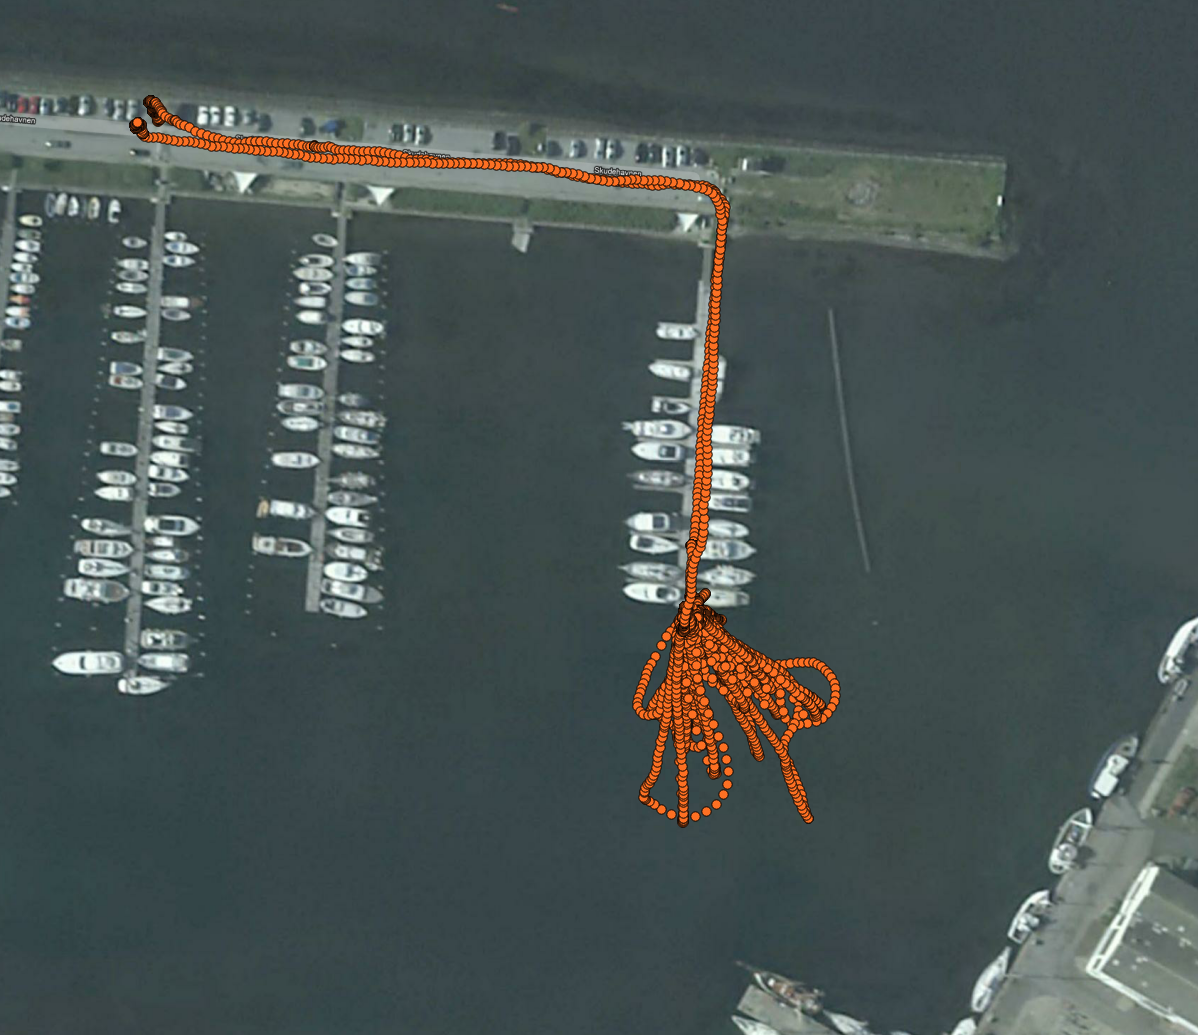
\includegraphics[width=\textwidth]{img/maidenVoyage/pointsOnMap}
	\caption{Manual control: GPS measurements with map} 
	\label{fig:pointsOnMap}
	\end{figure}

\begin{figure}[htpb]
	\centering
	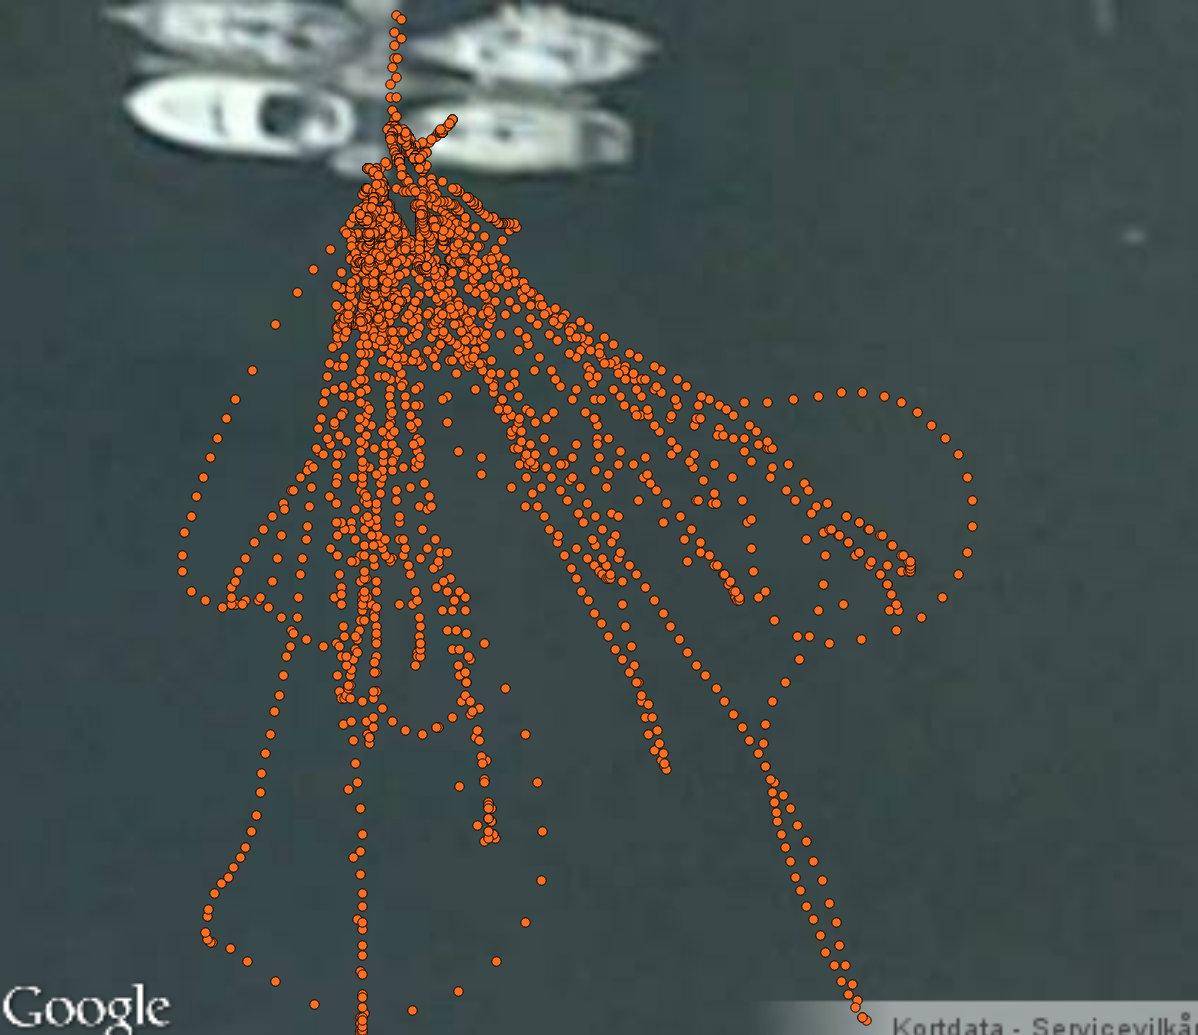
\includegraphics[width=\textwidth]{img/maidenVoyage/pointsOnMapZoom}
	\caption{Manual control: GPS measurements with map, zoom in} 
	\label{fig:pointsOnMap2}
\end{figure}

The boat was sealed with a lid and weighted with around 1.5 kg of lead in order to keep it as low in the water as possible, so that the propellers would not suck air in. Then a Python script was used which, when pressing "forward" or "back" would tell both motors to go faster of slower. The left arrow would increase the left propeller speed and would turn the right one down and vice versa. In this way, we were able to have basic control of the ship and test it. Space was used as an "emergency stop".

In pictures \vref{fig:pointsOnMap} and \vref{fig:pointsOnMap2} the data obtained from the GPS sensor during this trip is plotted on top of an Open Street map of the marina in which the tests took place. They begin in the top left of the picture, where we took the boat out of the car and walked to the water, then all the dots are the GPS messages received while performing sailing tests.

\begin{figure}[htpb]
	\centering
	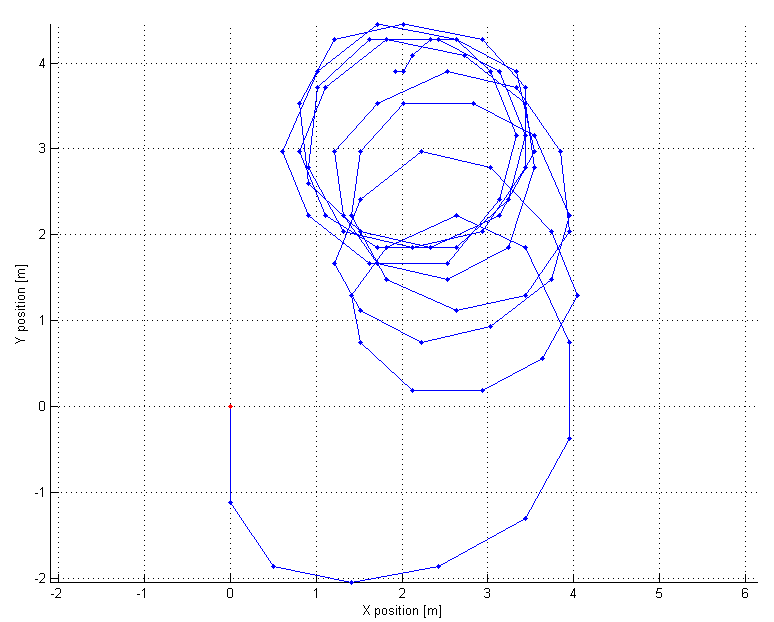
\includegraphics[width=\textwidth]{img/maidenVoyage/ship_turning2}
	\caption{GPS measurements of ship turning as logged by the LLI during maiden voyage} 
	\label{fig:ship_turning2}
\end{figure}

\begin{figure}[htpb]
	\centering
	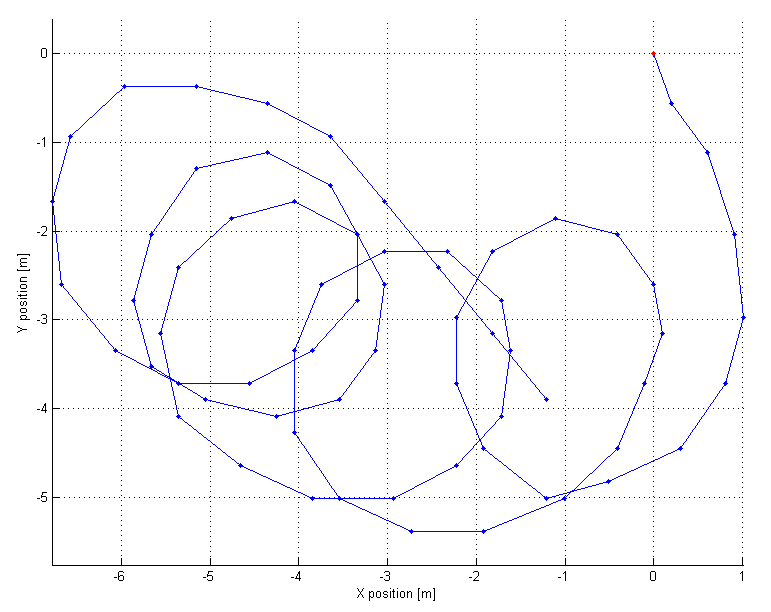
\includegraphics[width=\textwidth]{img/maidenVoyage/ship_turning}
	\caption{GPS measurements of ship turning as logged by the LLI during maiden voyage} 
	\label{fig:ship_turning}  
\end{figure}

Both Figure \vref{fig:ship_turning2} and \vref{fig:ship_turning} represent the ship in a continuous spiral. The turning radius will depend on the difference between the two motor speeds. It can be seen from the figures that this radius can be as small as 1 meter, which is a very good response. The red dot at (0, 0) represents the starting point.

The first wet test was also helpful in calibrating the control algorithm by noting that the motors are very powerful and that they should never be used at a very high throttle. Also, the motor controllers have some tolerance, meaning that the motors actually started turning forward at +10\% and reversing at -10\% of the available control signal. This hysteresis may induce jerks in the boat if not properly compensated because of overcompensating.



